\documentclass[11pt]{article}

\pdfobjcompresslevel=3    % compress PDF objects
\pdfcompresslevel=9       % compress streams more (0..9)
\pdfminorversion=4


\usepackage[utf8]{inputenc} % remove if using XeLaTeX or LuaLaTeX
\usepackage[T1]{fontenc}

% Layout & graphics
\usepackage[a4paper, total={7.5in, 9in}]{geometry}
\usepackage{graphicx}              % images
\usepackage[dvipsnames,table]{xcolor} % single xcolor invocation (keeps table option)

% Math & symbols
\usepackage{amsmath}
\usepackage{amssymb}
\usepackage{gensymb}

% Typography & layout helpers
\usepackage{microtype}
\usepackage{float}                 % [H] placement
\usepackage{caption}
\usepackage{subcaption}            % modern subfigure support (do NOT load subfig)
\usepackage{multirow}
\usepackage{titlesec}

\usepackage{lmodern}
\usepackage{microtype}

\definecolor{xppblue}{RGB}{37, 150, 190}

\begin{document}

\begin{table}[h]
\centering
\scalebox{1.5}{
\begin{tabular}{|ccll|cl|}
\hline
\multicolumn{4}{|c|}{SPRAWOZDANIE Z LABORATORIUM}                                                                                                                            & \multicolumn{2}{c|}{\multirow{2}{*}{\begin{tabular}[c]{@{}c@{}}rok akademicki:\\ 2024/25\end{tabular}}} \\ \cline{1-4}
\multicolumn{4}{|c|}{\textbf{Układy elektroniki użytkowej}}                                                                                                                          & \multicolumn{2}{c|}{}                                                                                   \\ \hline
\multicolumn{4}{|c|}{\multirow{2}{*}{\textit{Akwizycja danych w LabVIEW}}}                                                                                           & \multicolumn{2}{c|}{\multirow{2}{*}{czwartek 8:00}}                                                \\
\multicolumn{4}{|c|}{}                                                                                                                                                       & \multicolumn{2}{c|}{}                                                                                   \\ \hline
\multicolumn{1}{|c|}{WARiE, AiR, sem 5}          & \multicolumn{3}{c|}{\multirow{4}{*}{\begin{tabular}[c]{@{}c@{}}1. Mateusz Banaszak\\ \underline{2. Jan Andrzejewski}\\3. Ignacy Baniowski\\4.Bartosz Bacik\end{tabular}}} & \multicolumn{2}{l|}{\multirow{2}{*}{Punkty:}}                                                           \\ \cline{1-1}

\multicolumn{1}{|c|}{8.10.2025}                   & \multicolumn{3}{c|}{}                                                                                                   & \multicolumn{2}{l|}{}                                                                                   \\ \hline
\end{tabular}
}
\end{table}
\vspace{3\baselineskip}


\section{Sprzęt}
\begin{table}[H]
\centering
\begin{tabular}{lllll}
\cline{1-4}
\multicolumn{1}{|l|}{nr. stanowiska} & \multicolumn{1}{l|}{nr. Elvisa} & \multicolumn{1}{l|}{płyta prototypowa} & \multicolumn{1}{l|}{elementy} &  \\ \cline{1-4}
\multicolumn{1}{|l|}{2}               & \multicolumn{1}{l|}{2}           & \multicolumn{1}{l|}{}                  & \multicolumn{1}{l|}{}         &  \\ \cline{1-4}
\end{tabular}
\end{table}

\section{Ćwiczenie}
\subsection{Generacja sygnałów}

\begin{table}[H]
\centering
\begin{tabular}{|p{5cm}|p{5cm}|}
\hline
Bloki sterujące sprzętem & Bloki realizowane programowo \\ \hline
bezpośrednio wchodzą w interakcje z elementami umieszczonymi na płycie Elvis &  realizują funkcje wykonywane za pomocą procesora komputera i ich wyniki są przechowywane w pamięci \\ \hline
\end{tabular}
\end{table}


\begin{figure}[H]
    \centering
    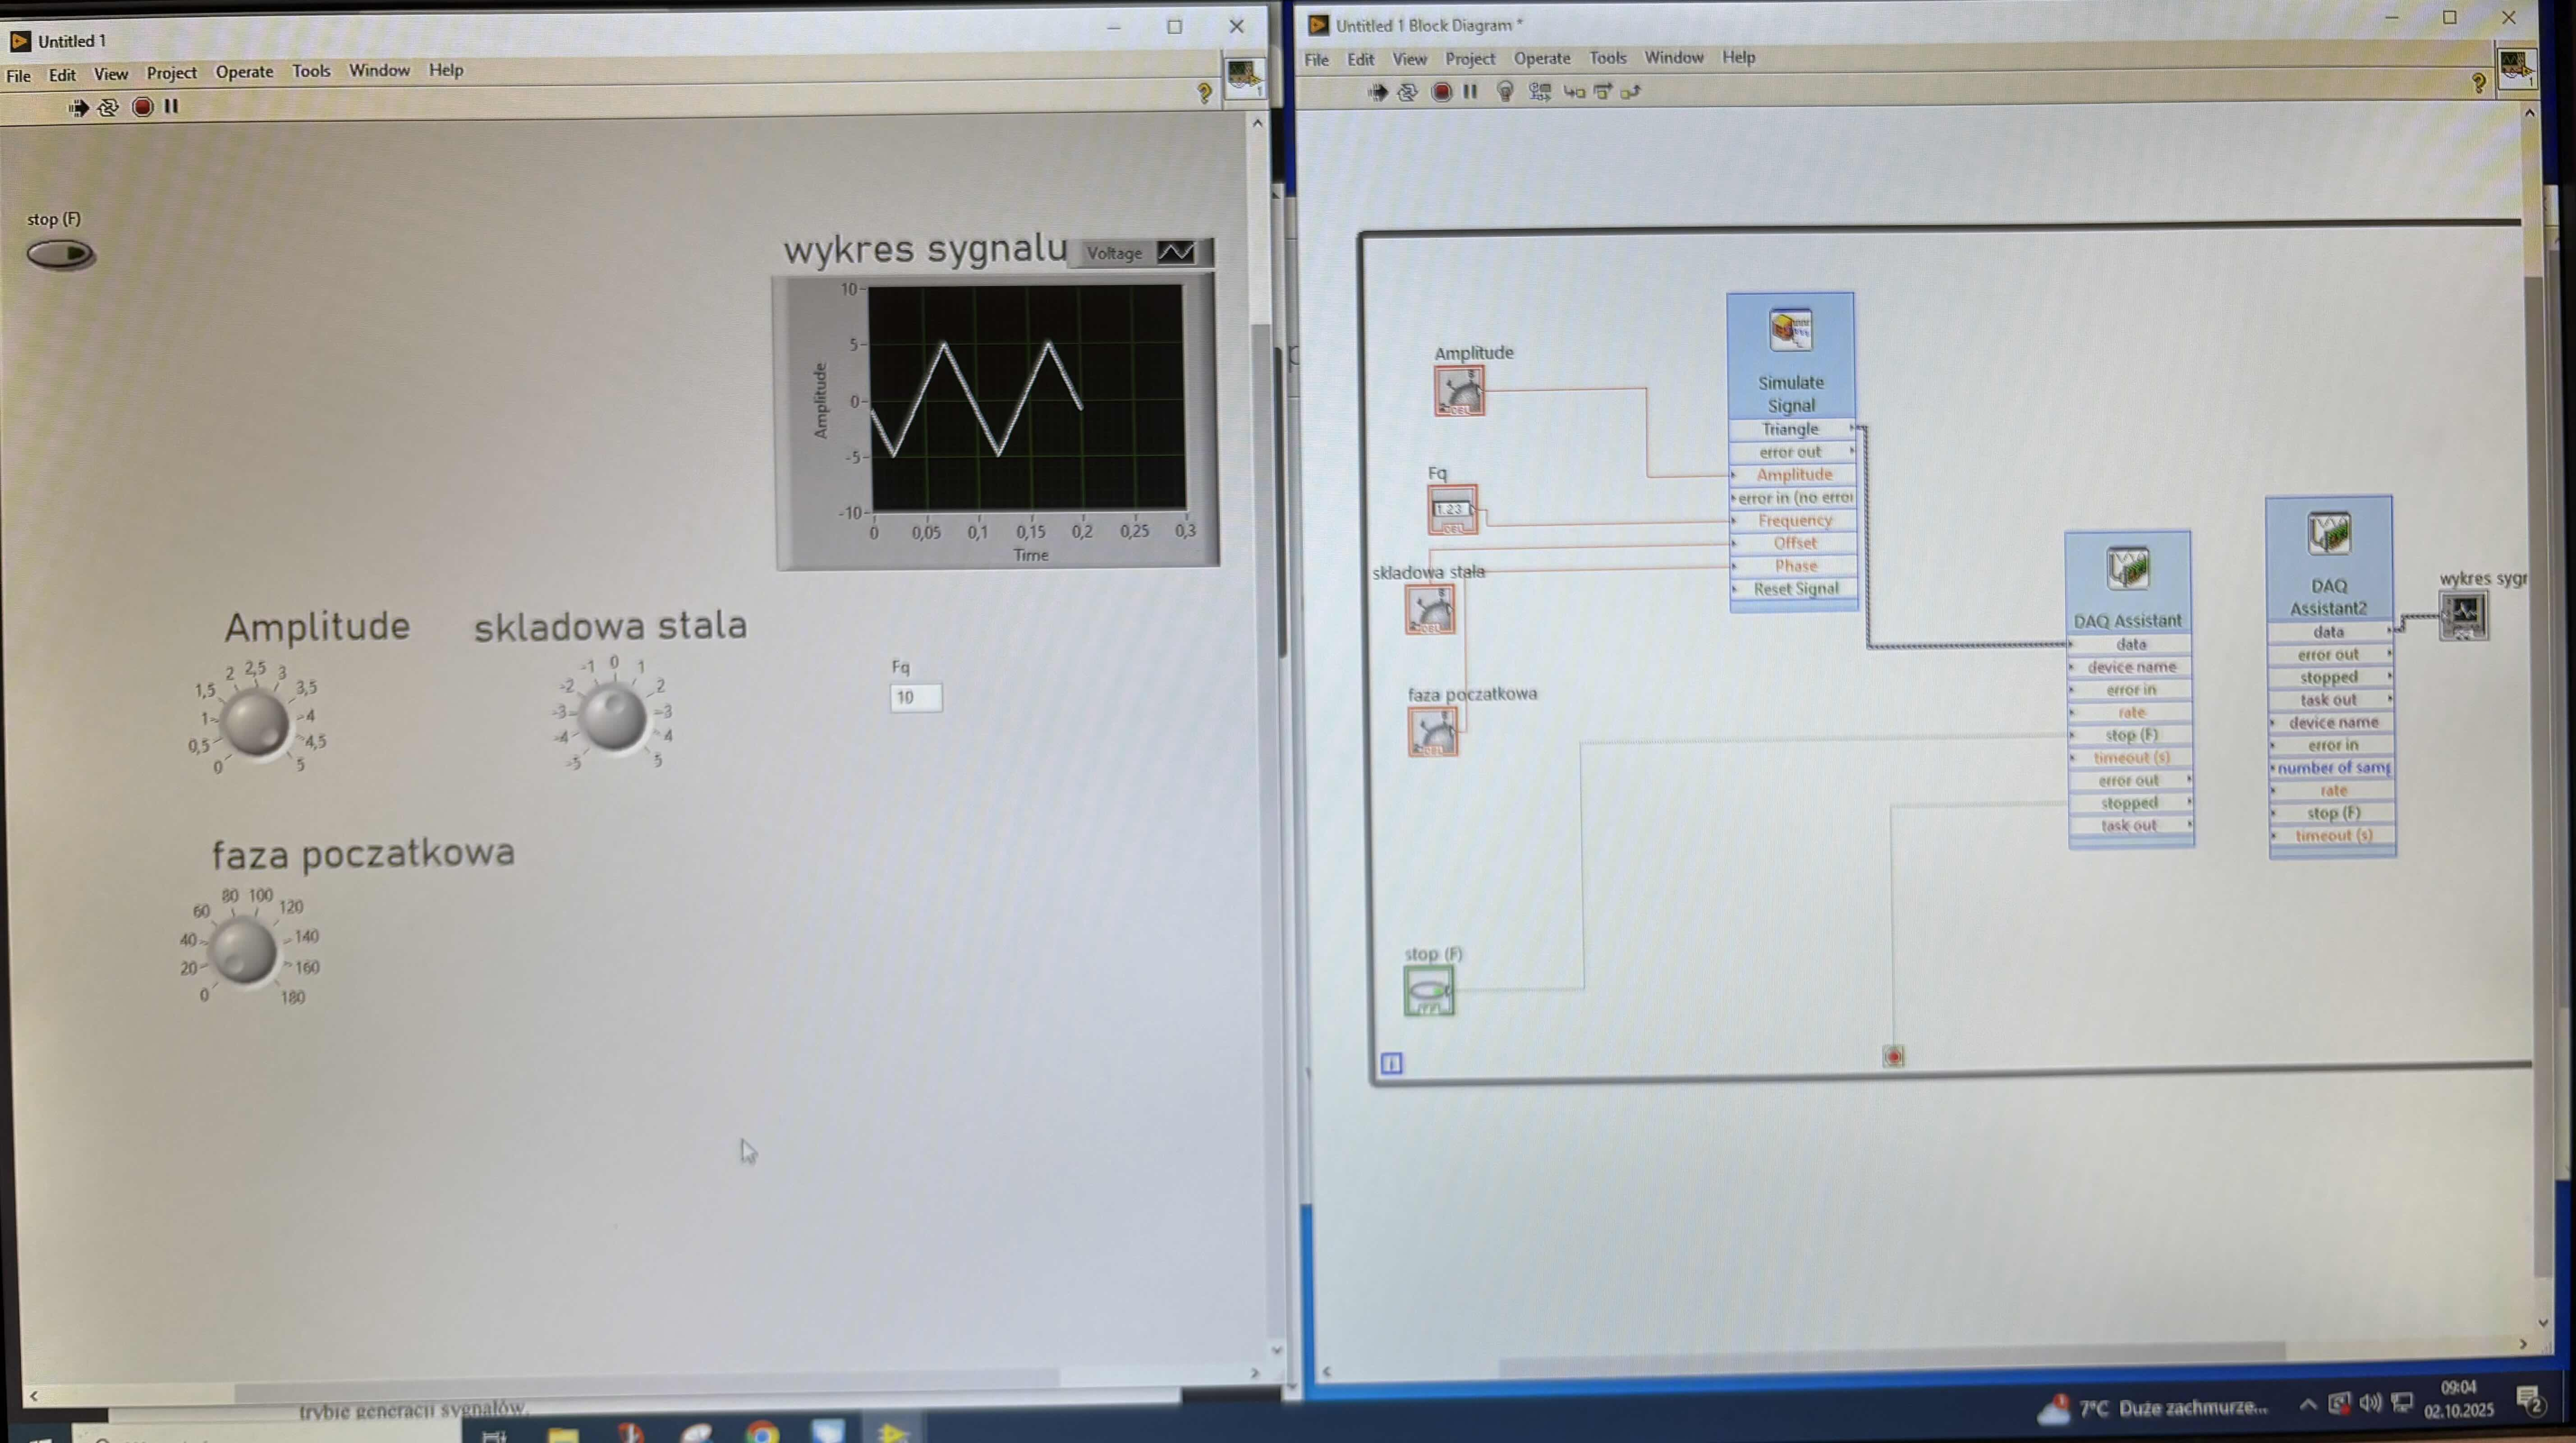
\includegraphics[width=0.5\linewidth]{img/obraz1.jpg}
    \caption{Gotowy układ do generacji układów w LabVIEW}
    \label{fig:placeholder}
\end{figure}

\begin{figure}[H]
  \centering
  \begin{subfigure}{.48\textwidth}
    \centering
    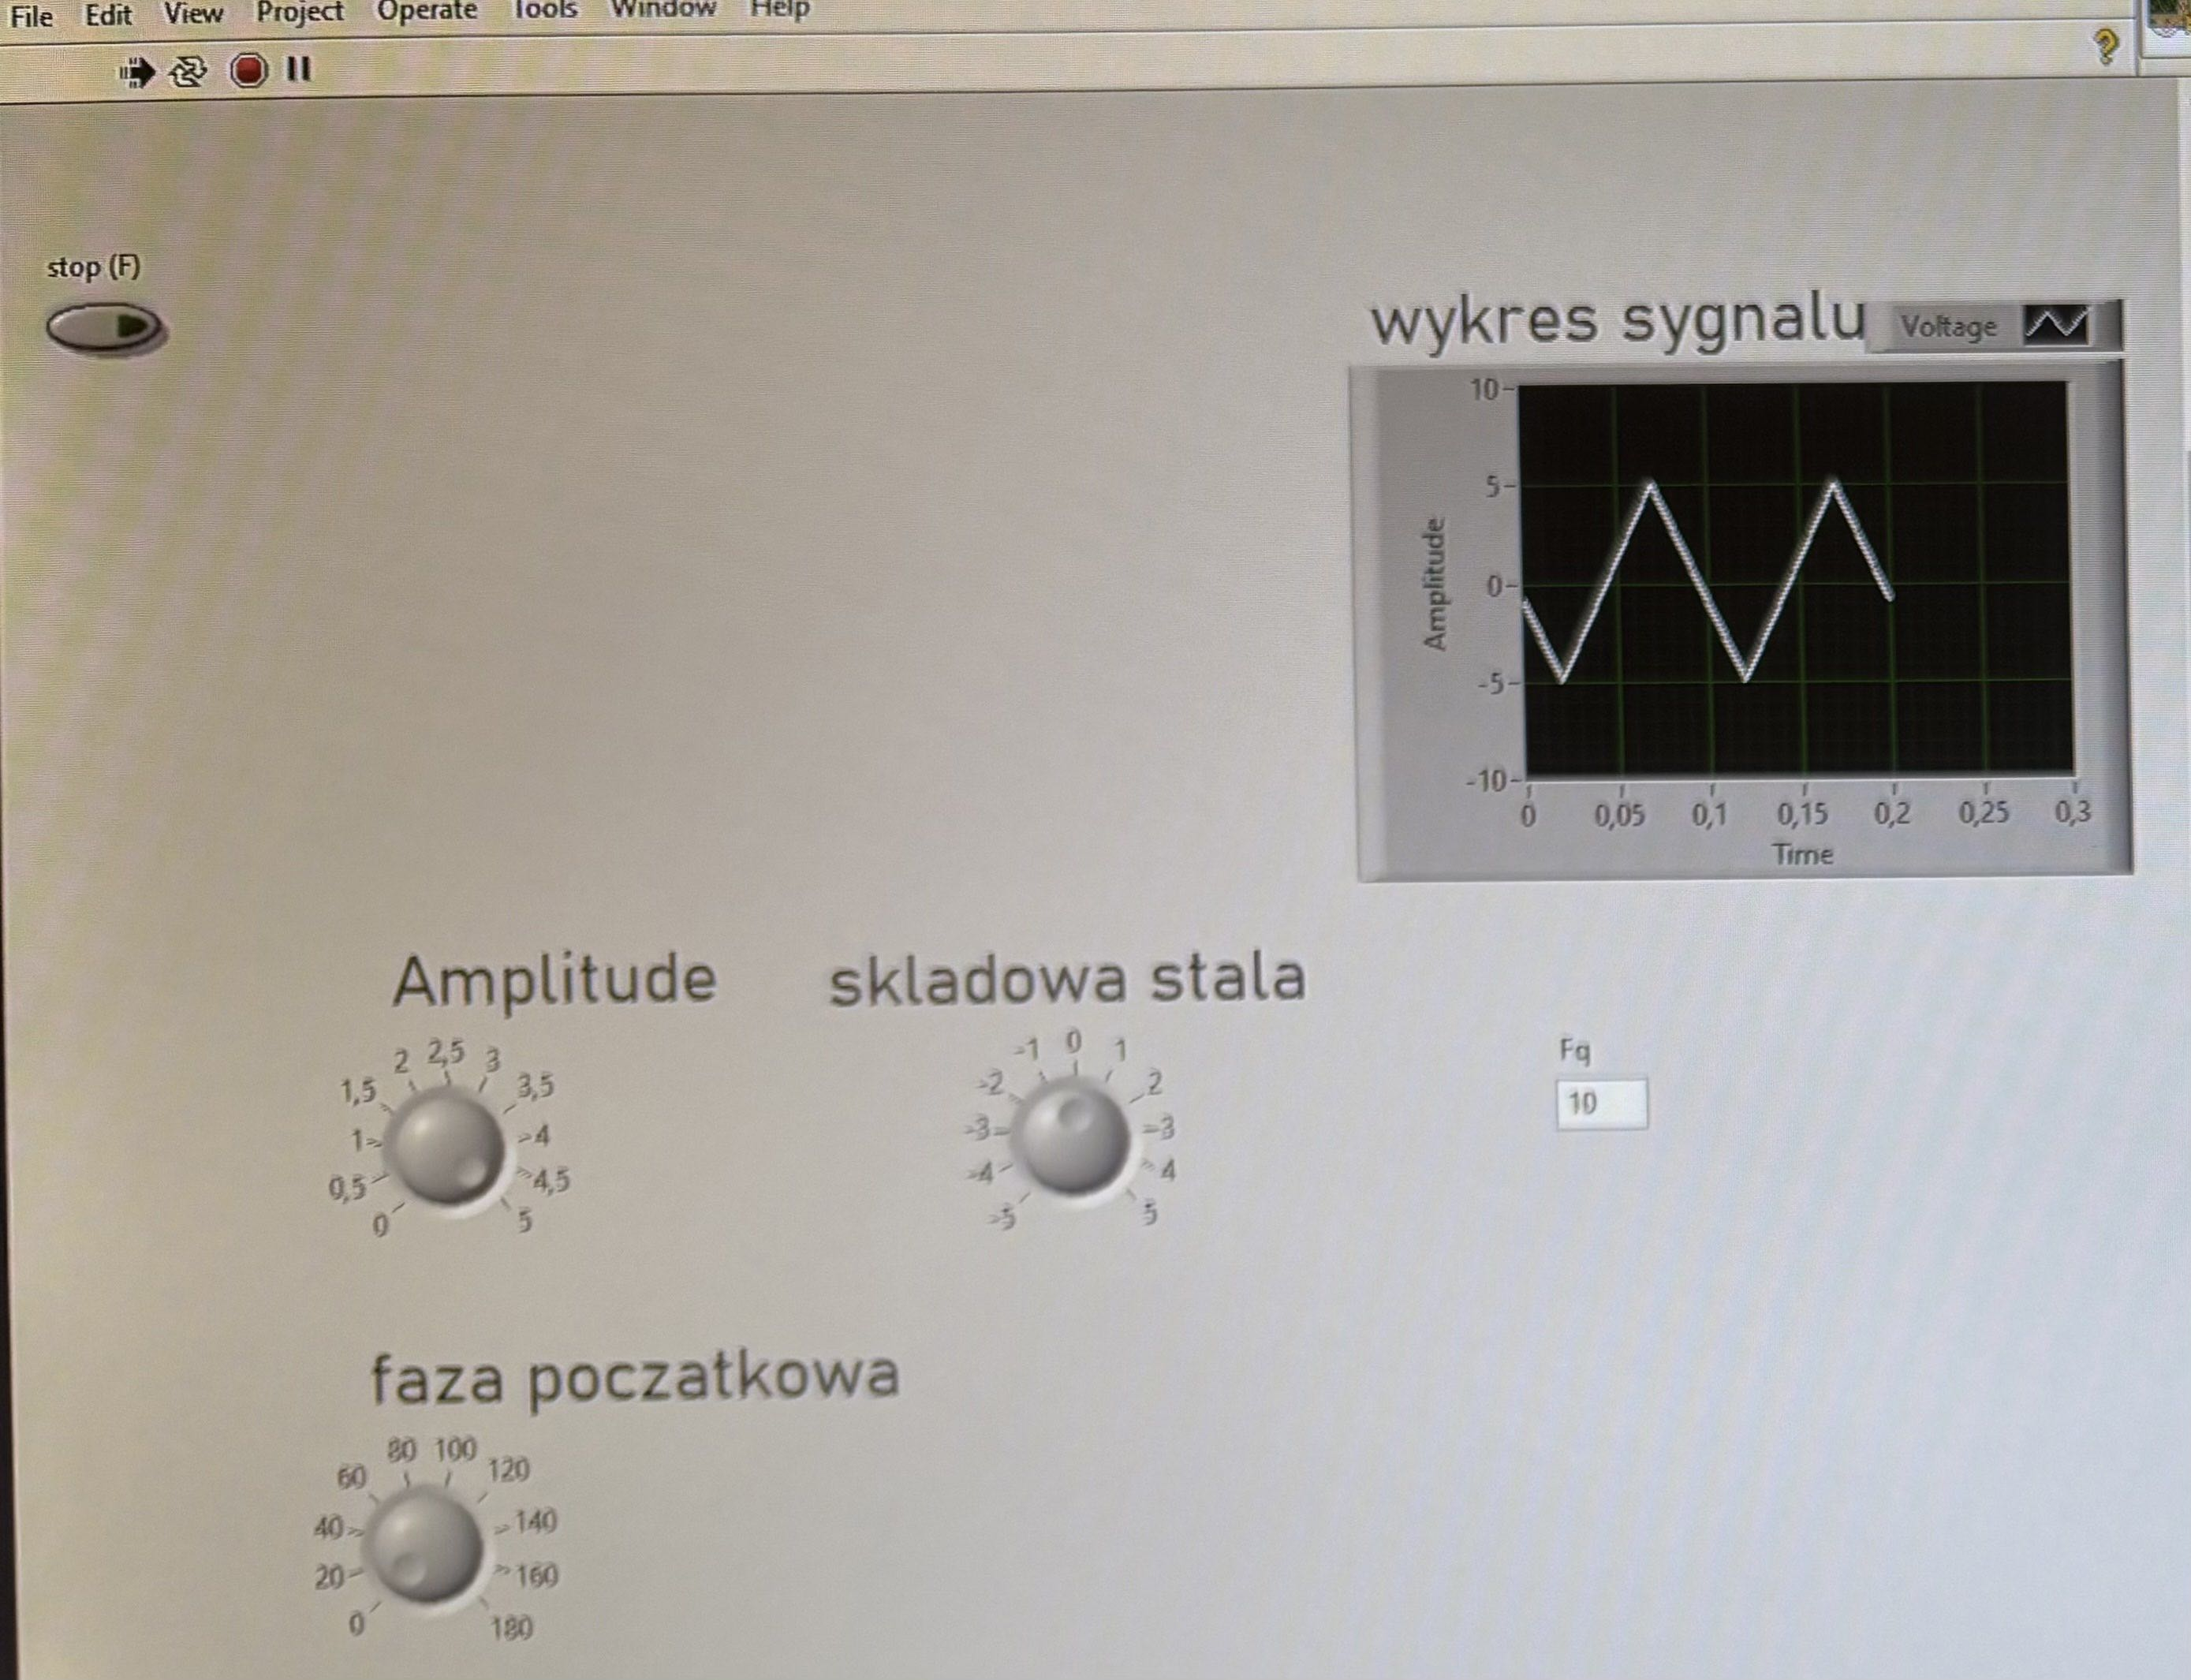
\includegraphics[width=\linewidth]{img/obraz2.jpg}
    \caption{sygnał trojkatny A=5V , f=10Hz, offset=0V, faza=0\degree}
    \label{fig:sub1}
  \end{subfigure}\hfill
  \begin{subfigure}{.48\textwidth}
    \centering
    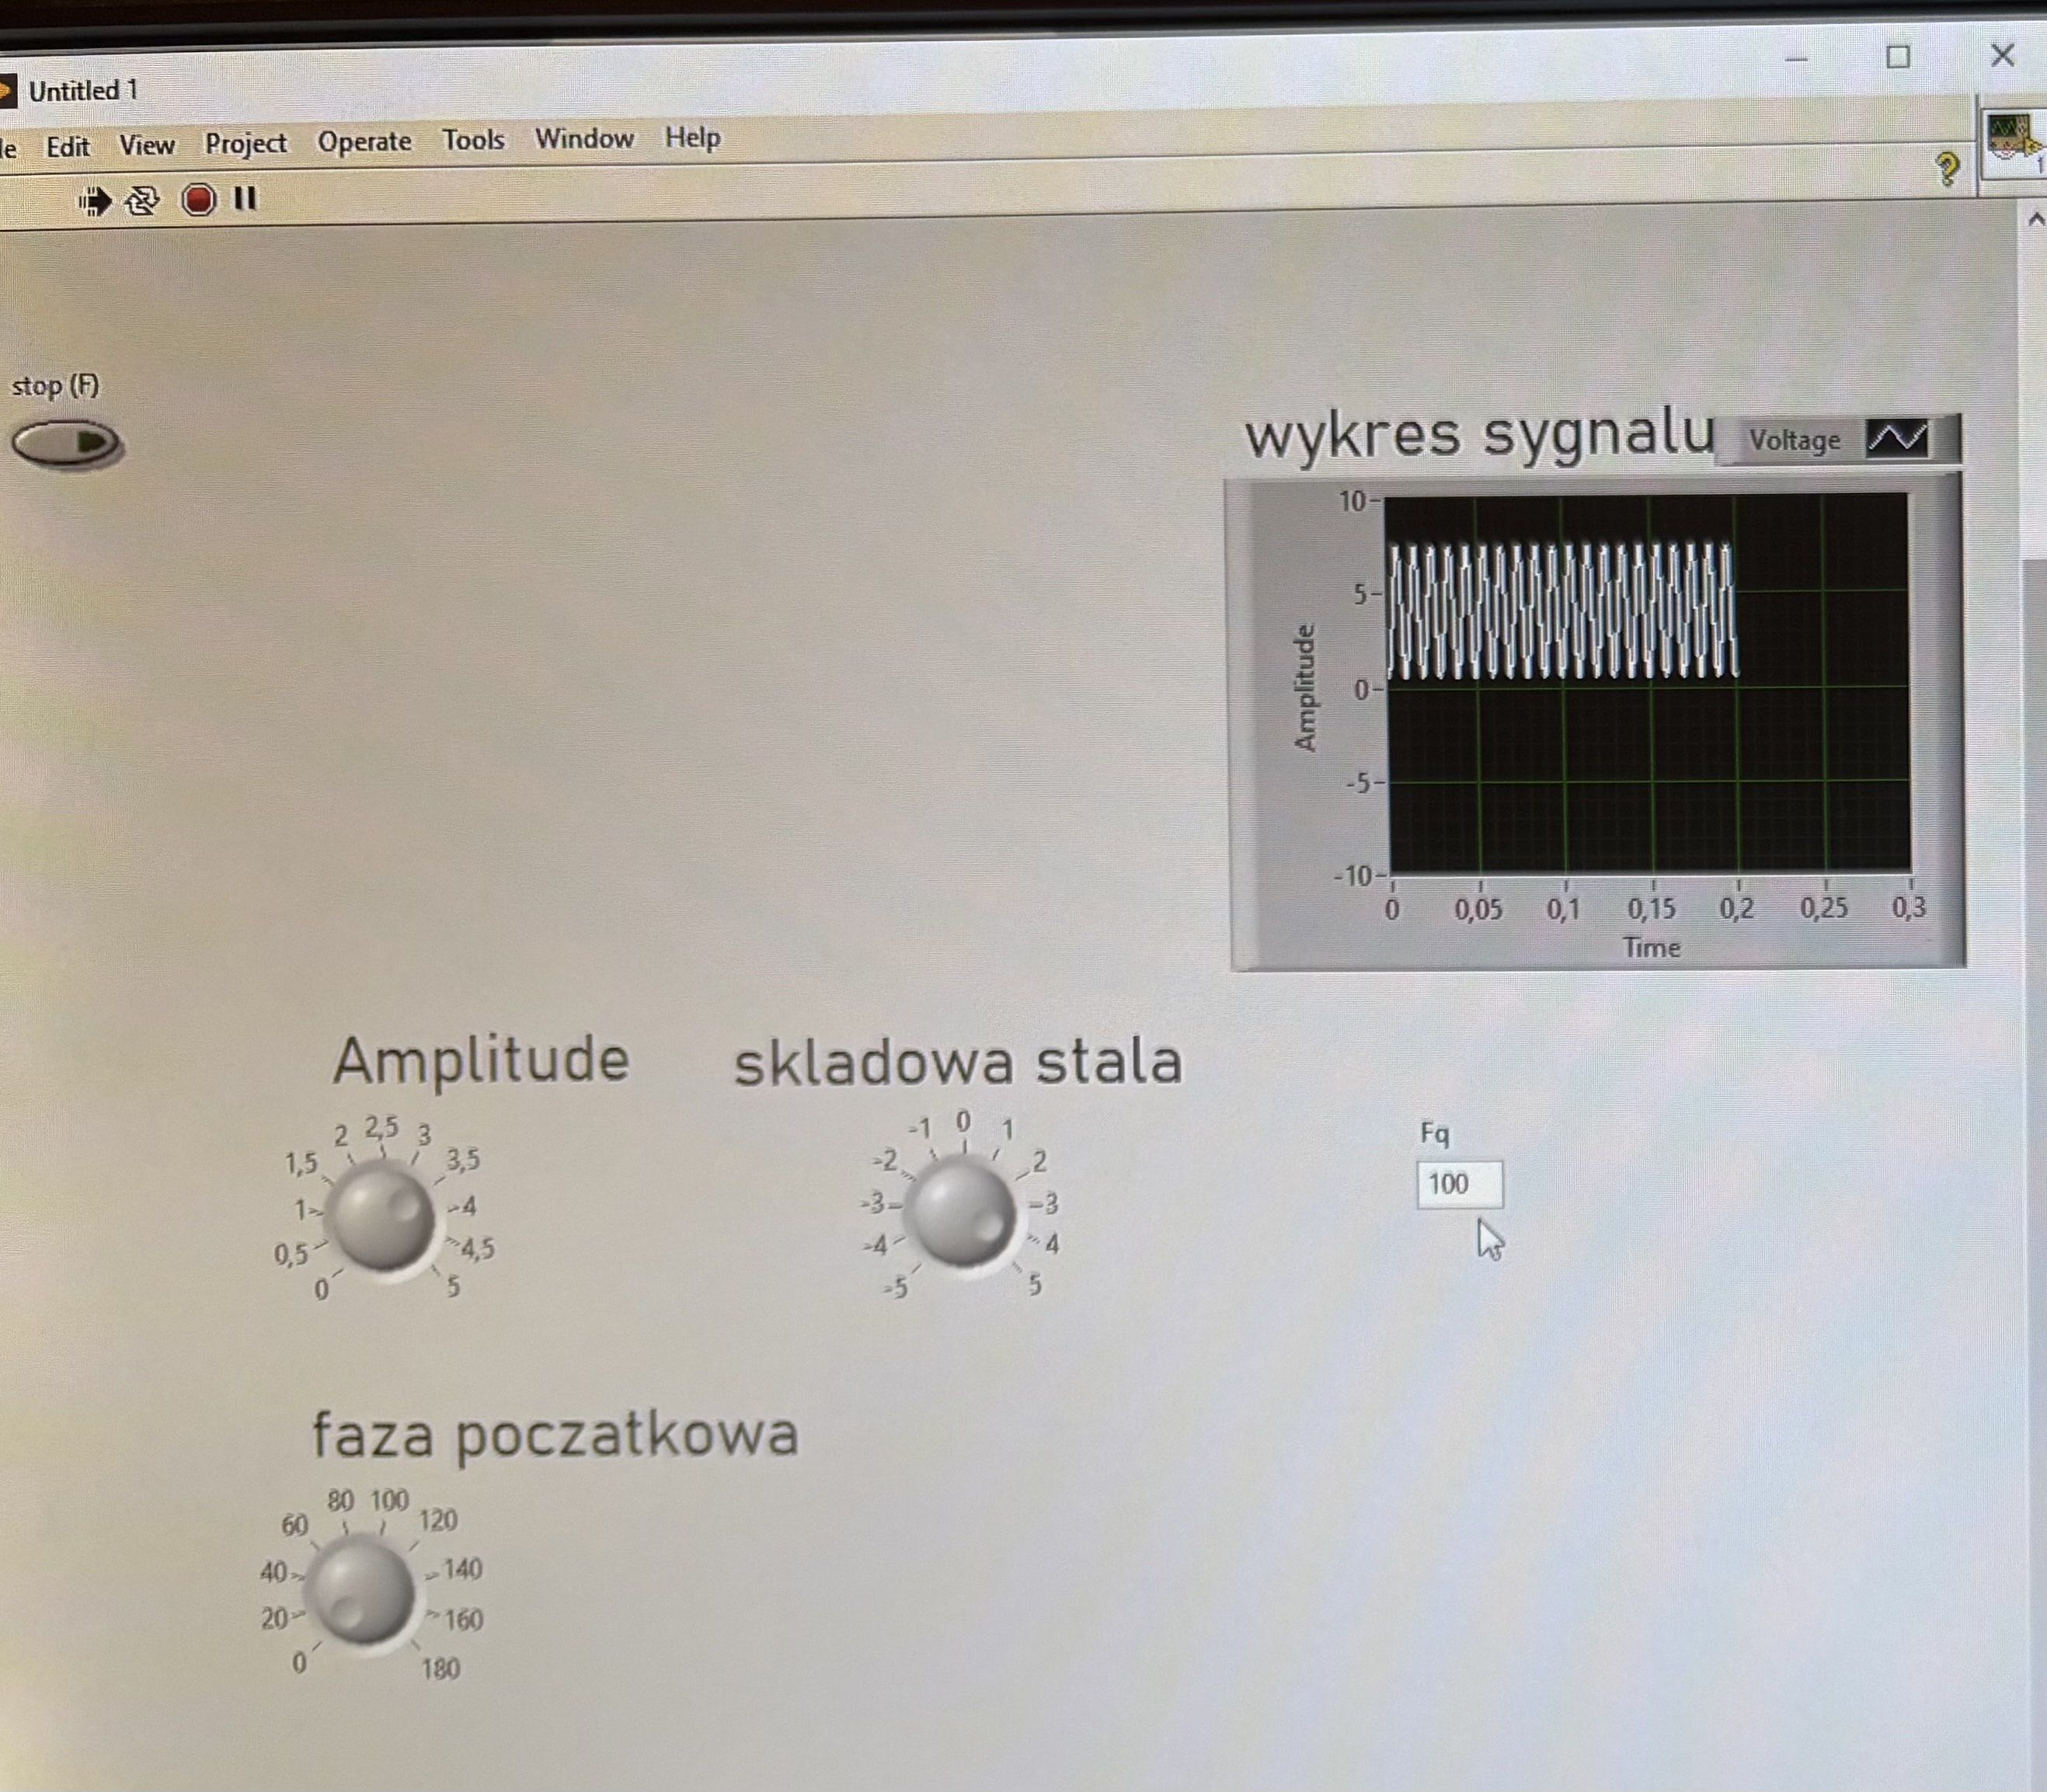
\includegraphics[width=\linewidth]{img/obraz3.jpg}
    \caption{sygnał sinusoidalny A=3.5V , f=100Hz, offset=5V, faza=0\degree}
    \label{fig:sub2}
  \end{subfigure}
  \begin{subfigure}{.48\textwidth}
    \centering
    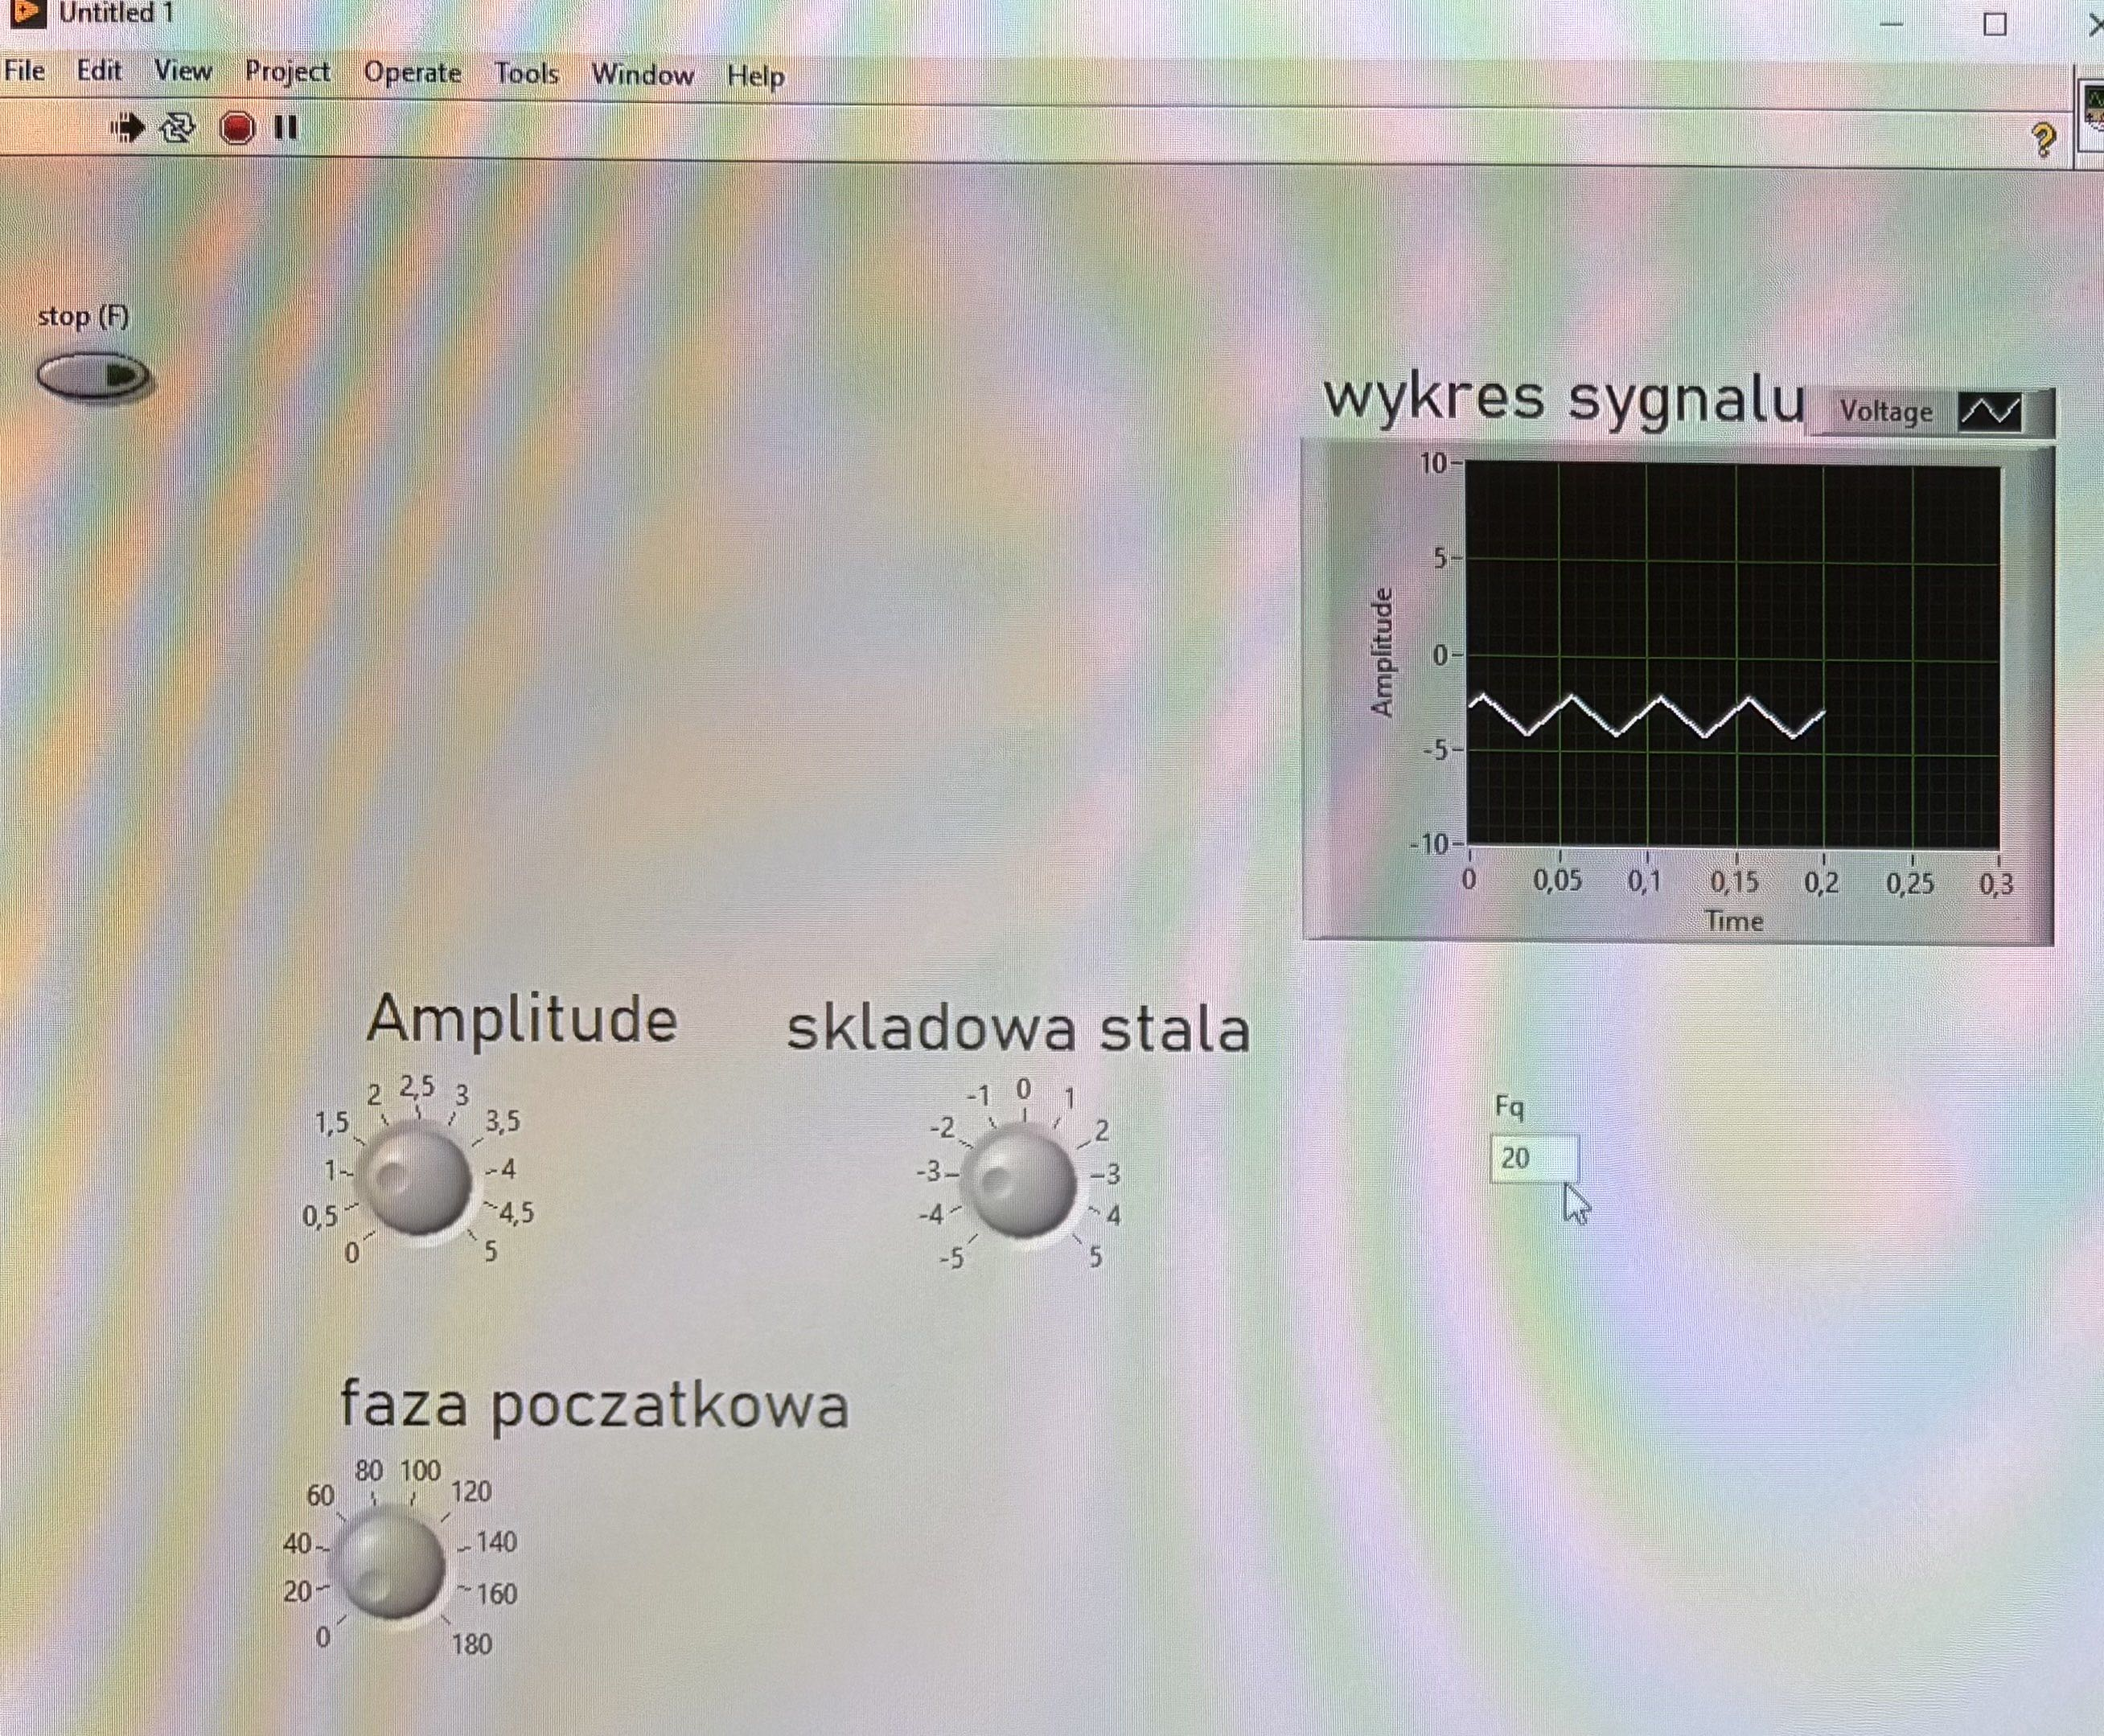
\includegraphics[width=\linewidth]{img/obraz4.jpg}
    \caption{sygnał tropjkatny A=1V , f=20Hz, offset=-3V, faza=0\degree}
    \label{fig:sub3}
  \end{subfigure}

  \caption{Przebiegi sygnałów wraz z nastawami}
  \label{fig:przebiegi}
\end{figure}


\subsection{Rejestracja sygnałów}
Zmodyfikowaliśmy połączenie na płycie tak ze pomiędzy wyjściem i wejściem nieodwracającym znajduje się kondensator 

\begin{figure}[H]
    \centering
    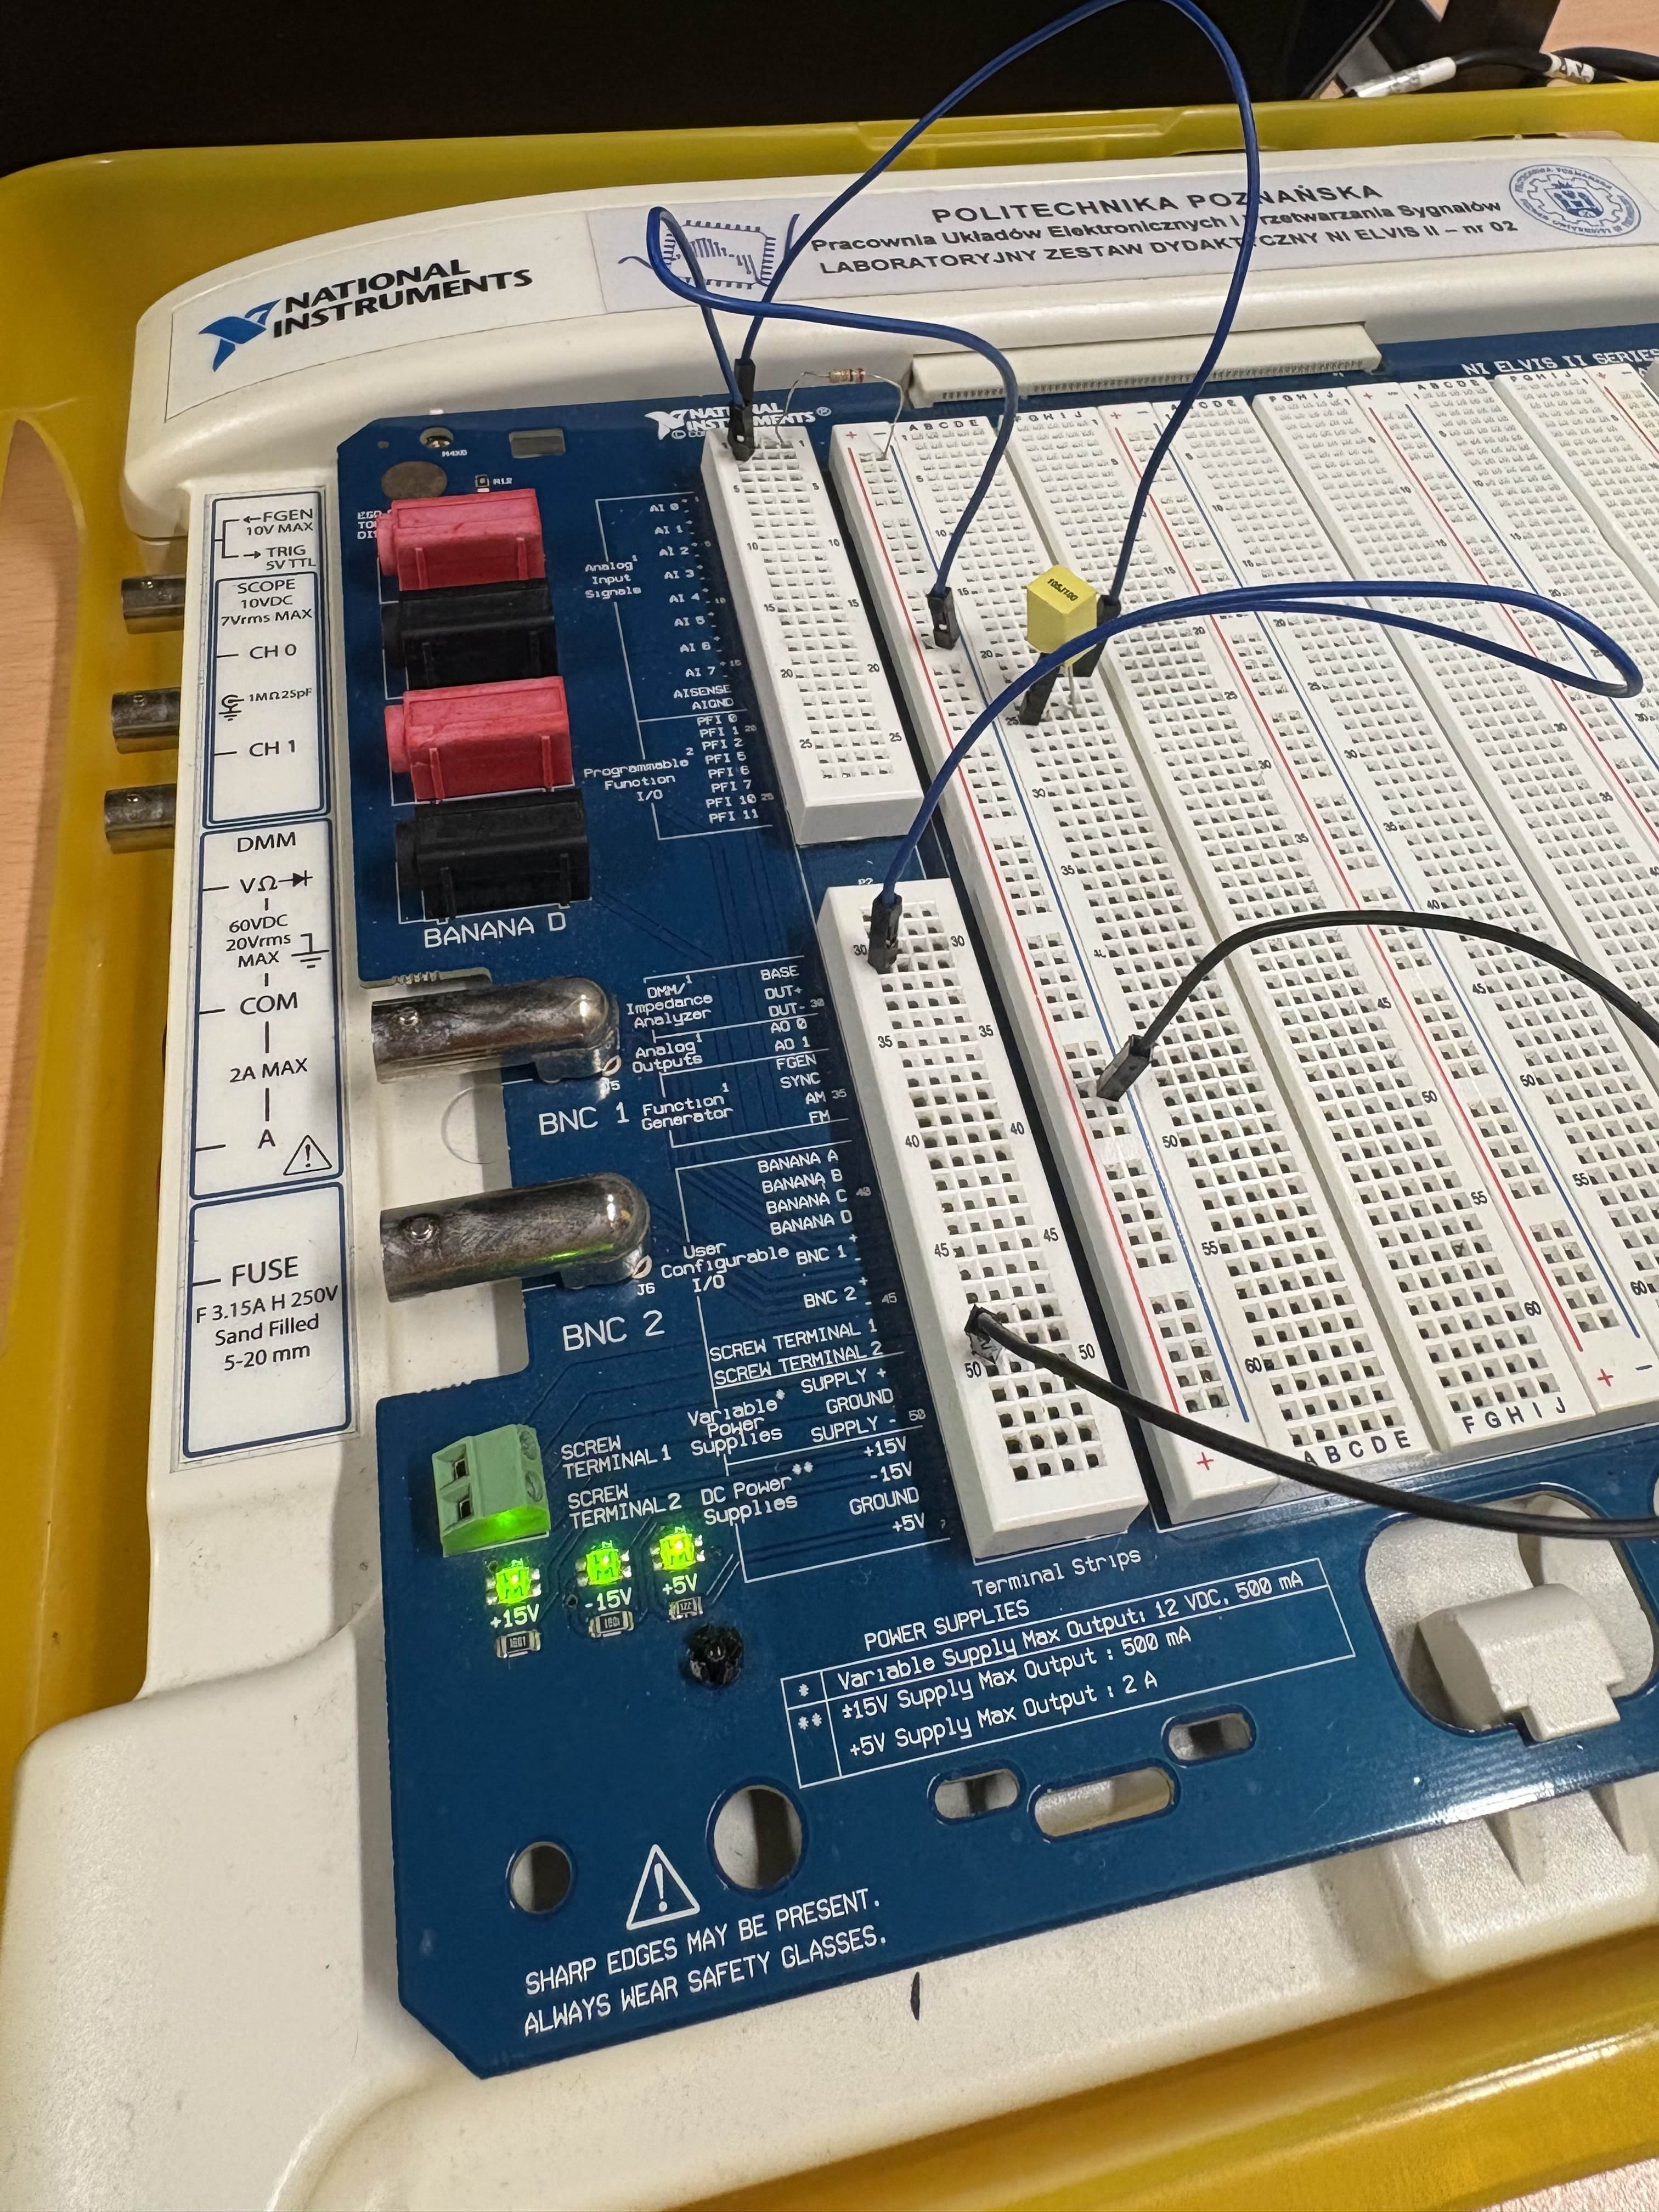
\includegraphics[width=0.3\linewidth]{img/obraz5.jpg}
    \caption{układ z kondensatorem}
    \label{fig:placeholder}
\end{figure}

\begin{figure}[H]
    \centering
    \includegraphics[width=0.5\linewidth]{img/image.png}
    \caption{Przebieg sygnału na wejściu i wyjściu}
    \label{fig:placeholder}
\end{figure}

Zbudowany przez nas układ pełni funkcje filtru górnoprzepustowego. Można to zaobserwowac przygladajac sie przebiegowi sygnału zarejestrowanego przez 
LabVIEW.

\begin{figure}[H]
    \centering
    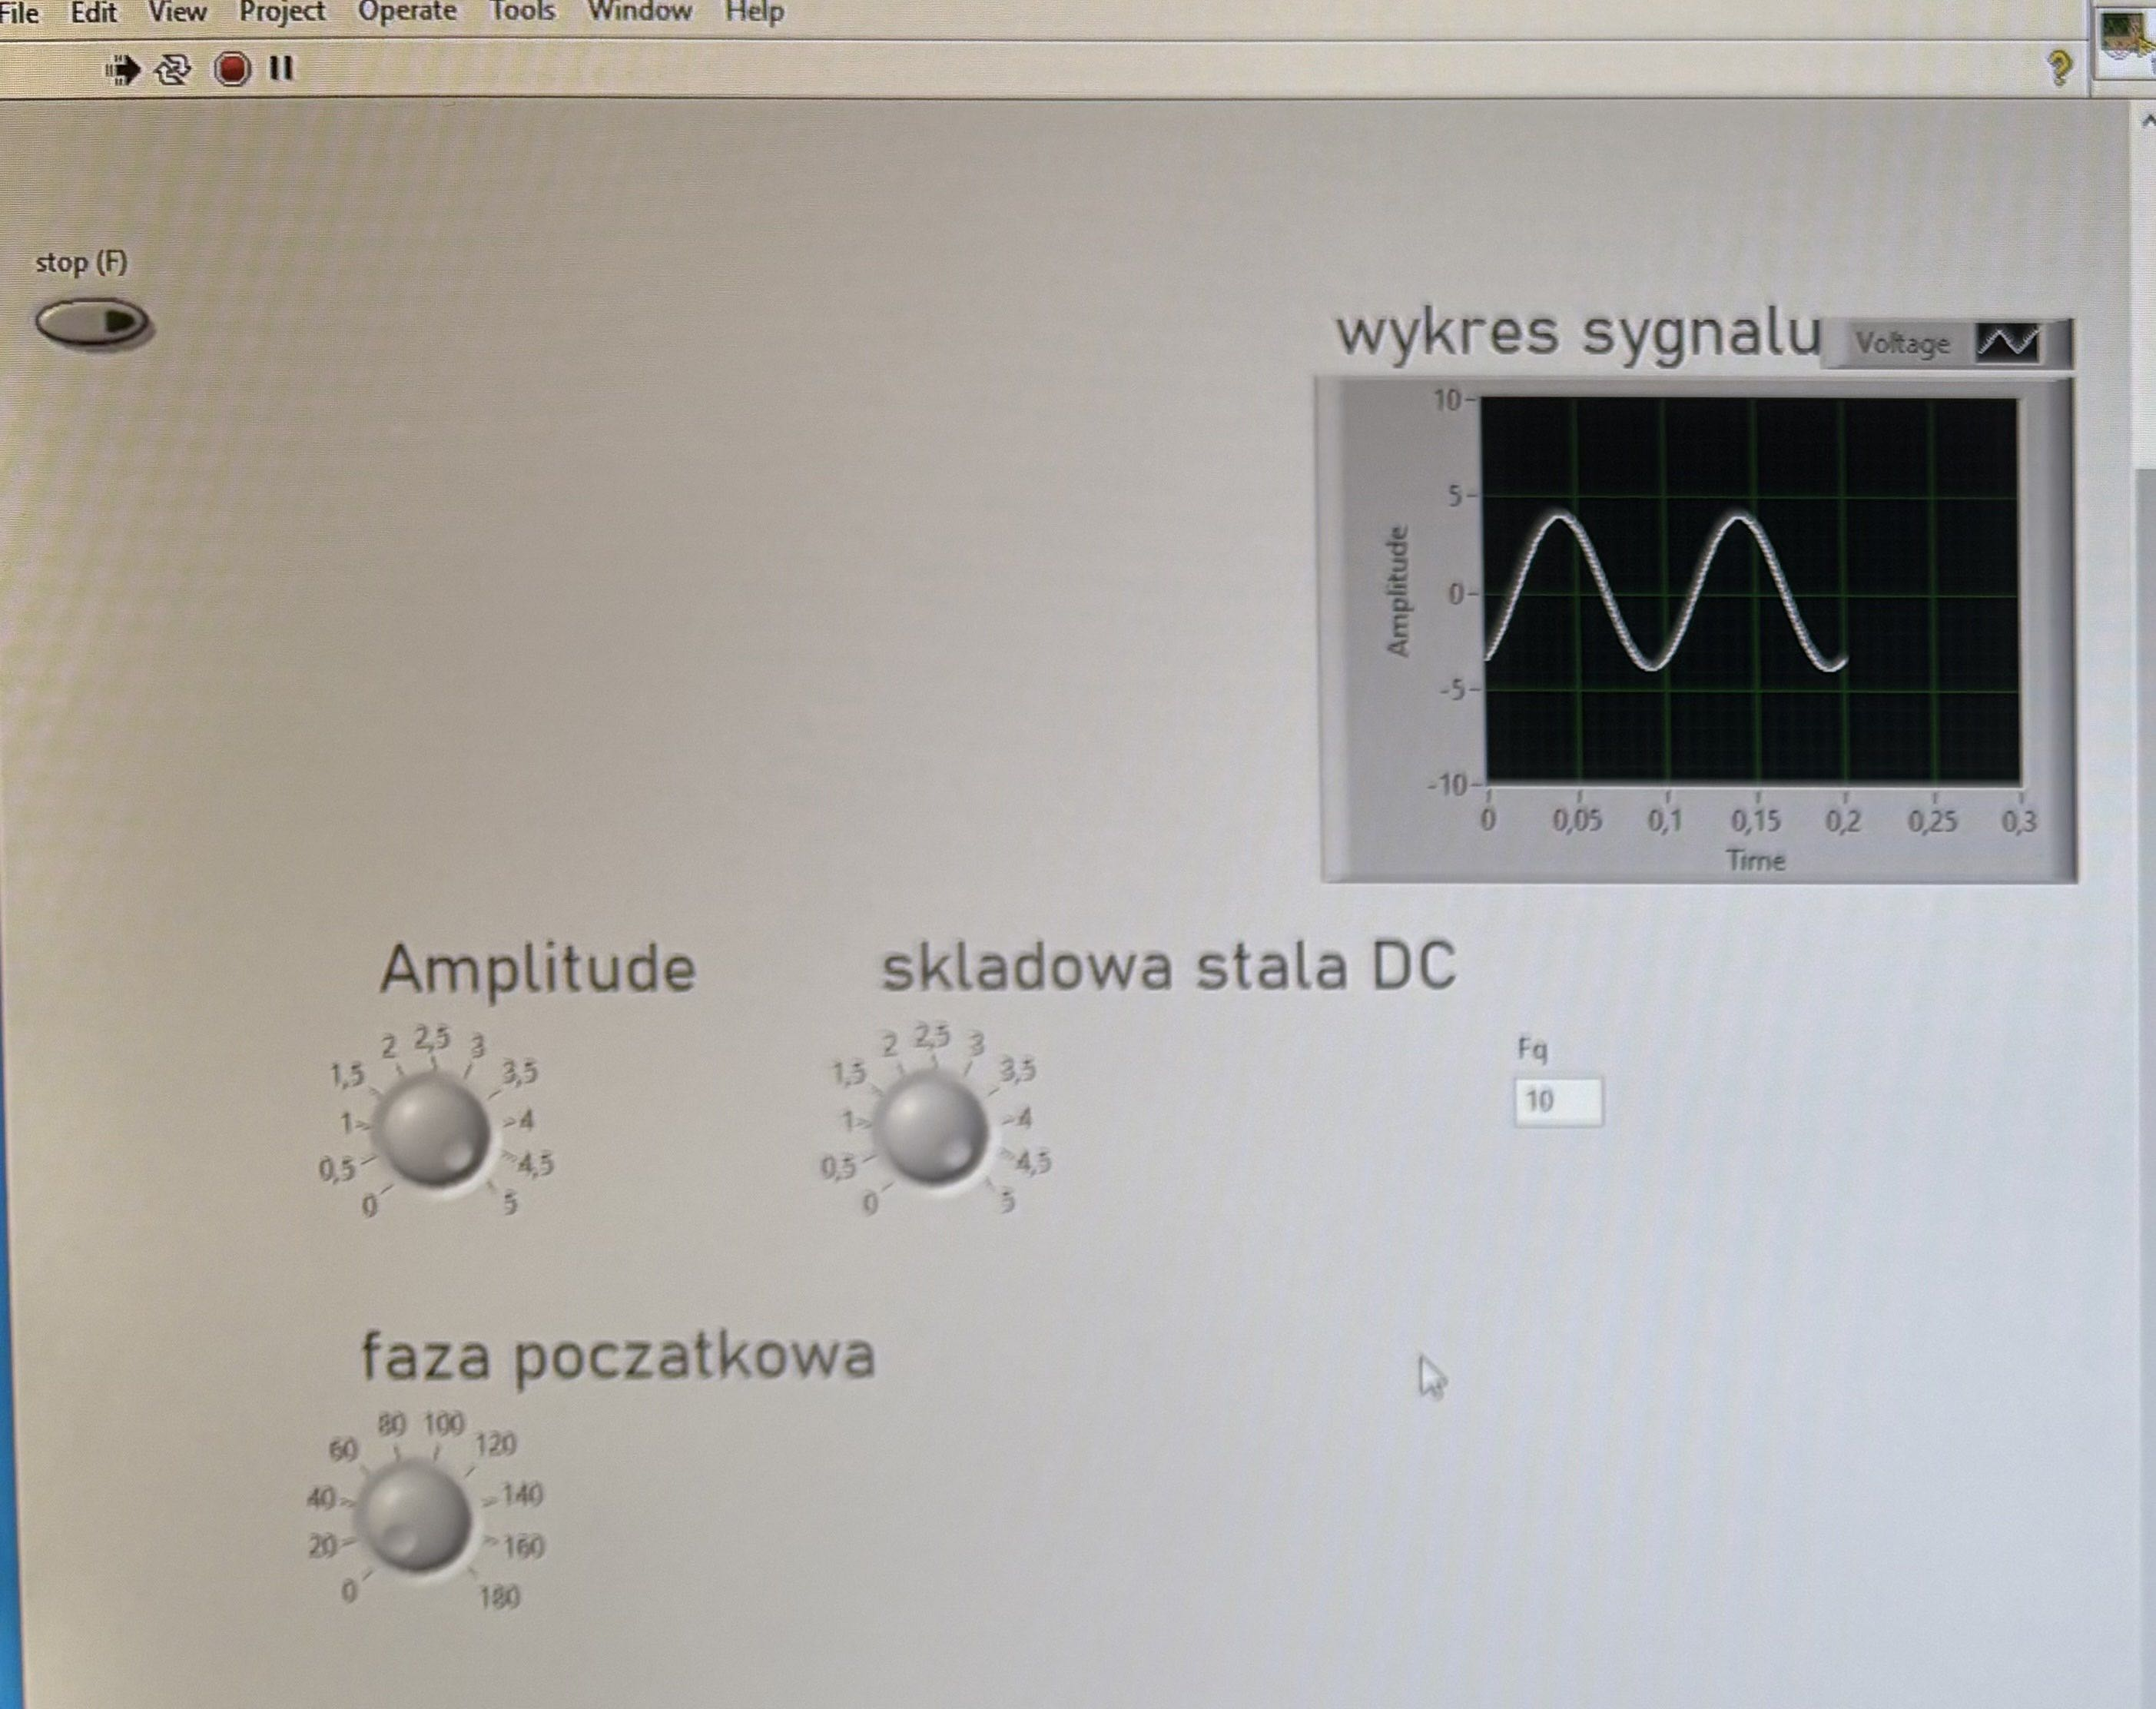
\includegraphics[width=0.5\linewidth]{img/image2.jpg}
    \caption{Przebieg sygnału poddanego filtracji}
    \label{fig:placeholder}
\end{figure}

Na przebiegu powyżej można zauważyć, że sygnał na wyjściu filtru nie ma w sobie składowej stałej. Jest to spowodowane
 obecnością kondensatora, który pełni funkcje filtru górnoprzepustowego.

\section{Wnioski}
  W trakcie ćwiczenia skupiliśmy się na pracy w środowisku LabVIEW, które jest 
  narzędziem do graficznego programowania i akwizycji danych. Poznaliśmy podstawowe
   możliwości LabVIEW, takie jak tworzenie wirtualnych instrumentów (VI), obsługa 
   bloków wejścia/wyjścia, generacja i rejestracja sygnałów oraz wizualizacja danych
    w czasie rzeczywistym. Korzystajac z LabVIEW jestesmy w stanie w prosty wizualny sposob 
    przygotowac skomplikowane uklady do generacji i pomiarów sygnałów.



\end{document}

